\subsubsection{UC13 - Interazione con una pagina del prodotto}
\begin{itemize}
\item \textbf{Attori primari}: utente generico;
\item \textbf{Descrizione}: l'utente può interagire con la pagina del prodotto attraverso appositi strumenti;
\item \textbf{Scenario Principale}: l'utente si trova nella pagina di un prodotto ed ha a disposizione le seguenti funzionalità:
\begin{itemize}
\item visualizzazione di tutte le informazioni riguardanti il prodotto [\textbf{UC13.1}];
\item modifica della quantità selezionata del prodotto [\textbf{UC13.2}];
\item inserimento nel carrello del prodotto visualizzato [\textbf{UC13.3}].
\end{itemize}
\item \textbf{Precondizione}: l'utente si trova nella PDP\ped{G} corrispondente al prodotto desiderato;
\item \textbf{Postcondizione}: l'utente ha a disposizione varie funzionalità per interagire con il prodotto visualizzato e può procedere alla sua aggiunta al carrello.
\end{itemize}

\begin{figure}[H]
\centering
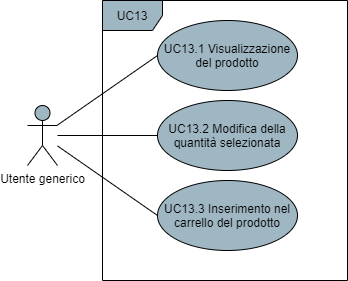
\includegraphics[scale=0.6]{res/UseCase/Immagini/InterazionePaginaProdotto}
\caption{Diagramma UML\ped{G} per UC13 - Interazione con una pagina del prodotto}
\end{figure}

\subsubsection{UC13.1 - Visualizzazione del prodotto}
\begin{itemize}
\item \textbf{Attori primari}: utente generico;
\item \textbf{Descrizione}: l'utente può visualizzare le seguenti informazioni che caratterizzano il prodotto:
\begin{itemize}
\item nome;
\item immagine;
\item descrizione;
\item prezzo;
\item tasse applicate;
\item quantità di prodotto selezionata (la quantità di default corrisponde ad 1).
\end{itemize}
\item \textbf{Scenario Principale}: l'utente visualizza le caratteristiche dell'oggetto descritto nella corrente PDP\ped{G};
\item \textbf{Precondizione}: l'utente ha cliccato sulla PDP\ped{G} dedicata al prodotto scelto;
\item \textbf{Postcondizione}: l'utente visualizza le informazioni relative al prodotto desiderato, con la possibilità di aggiungerlo al carrello.
\end{itemize}

\subsubsection{UC13.2 - Modifica della quantità selezionata}
\begin{itemize}
\item \textbf{Attori primari}: utente generico;
\item \textbf{Descrizione}: l'utente può modificare la quantità selezionata del prodotto, che di default è 1, modificando il campo apposito;
\item \textbf{Scenario Principale}: l'utente modifica la quantità selezionata del prodotto utilizzando l'apposito campo;
\item \textbf{Precondizione}: l'utente sta visualizzando il prodotto descritto nella PDP\ped{G};
\item \textbf{Postcondizione}: la quantità del prodotto visualizzato dall'utente è stata aggiornata al nuovo valore richiesto.
\end{itemize}

\subsubsection{UC13.3 - Inserimento nel carrello del prodotto visualizzato}
\begin{itemize}
\item \textbf{Attori primari}: utente generico;
\item \textbf{Descrizione}: l'utente può inserire il prodotto nel carrello, nella quantità desiderata, cliccando un apposito pulsante. La quantità di default del prodotto corrisponde ad 1;
\item \textbf{Scenario Principale}:
\begin{enumerate}
\item l'utente visualizza le informazioni del prodotto [\textbf{UC13.1}];
\item l'utente può modificare la quantità del prodotto attraverso un apposito campo [\textbf{UC13.2}];
\item l'utente preme il pulsante per l'inserimento del prodotto nel carrello.
\end{enumerate}
\item \textbf{Precondizione}: l'utente sta visualizzando le caratteristiche del prodotto presente nel catalogo digitale;
\item \textbf{Postcondizione}: l'utente ha inserito nel carrello il prodotto nella quantità da lui desiderata.
\end{itemize}